\songchapter{S}

%%%%%%%%%%%%%%%%%%%%%%%%%%%%%
\songsection{声音碎片}	\index{S!shengyinsuipian}

%%%%%%%%%%%%%%%%%%%
\subsection{优美的低于生活}

\begin{figure}[htp]
	\begin{center}
	  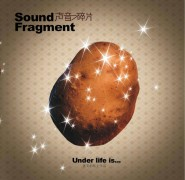
\includegraphics[scale = 0.80]{s/youmei}
% 	  \caption[labelInTOC]{优美的低于生活}
	  \label{fig:youmei}
	\end{center}
\end{figure}

\begin{songs}{}
  \beginsong{优美的低于生活}[index={优美的低于生活}]
	把歌声还给夜晚	\\
	把道路还给尽头	\\
	把果实还给种子	\\
	把飞翔还给天空	\\
	剩下的,让它们美好	\\
	从容的埋藏得更深	\\
	最后和纷乱的一切	\\
	都单纯的低于生活	\\
	吗咿呀咿呀咿呀	\\
	只要内心远过空旷	\\
	吗咿呀咿呀咿呀	\\
	梦到了丰饶的草原	\\
	\vspace{2ex}
	相爱吧,终有一散的人们	\\
	你失去的不过是童贞	\\
	等时光用尽了青春	\\
	你早已优美的在大街上溶化	\\
	吗咿呀咿呀咿呀	\\
	只要内心远过空旷	\\
	吗咿呀咿呀咿呀	\\
	梦到了丰饶的草原	\\
	\vspace{2ex}
	吗咿呀咿呀咿呀	\\
	只要内心远过空旷	\\
	吗咿呀咿呀咿呀	\\
	梦到了丰饶的草原	\\
  \endsong

  \beginsong{在时代华美的盛宴上}[index={在时代华美的盛宴上}]
	渐渐茫然的人们	\\
	已经忽略了悲喜	\\
	他们在河的两岸 目睹流失	\\
	在微凉的黄昏里	\\
	有人开始跳起舞	\\
	舞步划出的弧线 那么单纯	\\
	他们是如此得宁静	\\
	如此得骄傲	\\
	来不及去选择 就已惊慌	\\
	在时代华美的盛宴上	\\
	人群凌乱如草	\\
	不懂向内生长	\\
	看起来却那么美好	\\
	\vspace{2ex}
	厌倦是欢乐背后	\\
	唯一真实的伤口	\\
	最先倒下的少年 还面带微笑	\\
	没有人得到爱情	\\
	没有人选择离开	\\
	被惊扰的天空啊 一贫如洗	\\
	在时代华美的盛宴上	\\
	烟花迷乱如星	\\
	短暂的灿烂 让人群晕眩	\\
	在时光无尽的辽阔里	\\
	生命轻如尘埃	\\
	春天远去的消息	\\
	就让我们 泪如雨下	\\
	泪如雨下 泪如雨下	\\
	泪如雨 泪如雨下	\\
  \endsong
\end{songs}
